\documentclass{article}
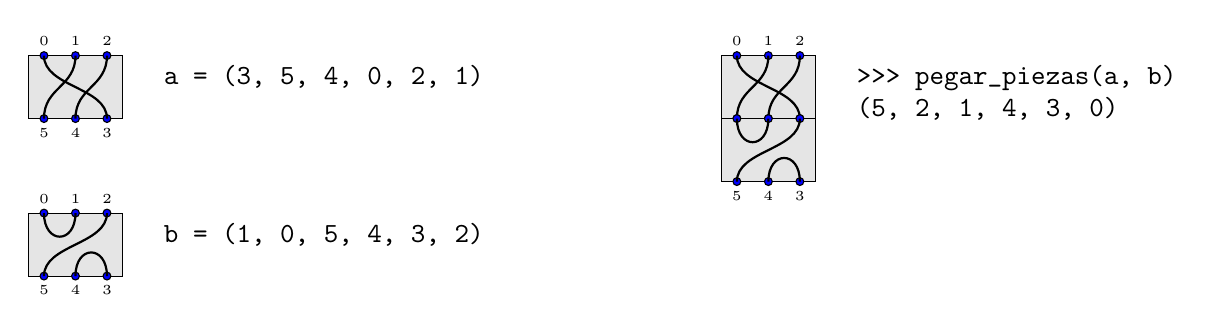
\begin{tikzpicture}[yscale=-1, scale=.4]

  \def\bottom{2}
  \def\top{0}

  \def\topnumbers{
    \foreach\x in {0, 1, 2}
      \node[anchor=south] at (\x + .5, \top) {\tiny \x};
  }
  \def\bottomnumbers{
    \foreach\x in {3, 4, 5}
      \node[anchor=north] at (5.5 - \x, \bottom) {\tiny \x};
  }

  \def\piece{%
    \draw[fill=black!10] (0, \top) rectangle ++(3, \bottom);
    \foreach \x in {.5, 1.5, 2.5}
      \foreach \y in {\bottom, \top}
        \node[draw, fill=blue, circle, inner sep=1pt] at (\x, \y) {};
  }

  \begin{scope}[yshift=0]
    \piece
    \topnumbers
    \bottomnumbers
    \draw[thick] (0.5, \bottom) .. controls (0.5, 1) and (1.5, 1) .. (1.5, \top);
    \draw[thick] (1.5, \bottom) .. controls (1.5, 1) and (2.5, 1) .. (2.5, \top);
    \draw[thick] (2.5, \bottom) .. controls (2.5, 1) and (0.5, 1) .. (0.5, \top);
    \node[anchor=north west] at (4, 0) {\texttt{a = (3, 5, 4, 0, 2, 1)}};
  \end{scope}

  \begin{scope}[yshift=5cm]
    \piece
    \topnumbers
    \bottomnumbers
    \draw[thick] (0.5, \top)    .. controls (0.5, 1) and (1.5, 1) .. (1.5, \top);
    \draw[thick] (1.5, \bottom) .. controls (1.5, 1) and (2.5, 1) .. (2.5, \bottom);
    \draw[thick] (2.5, \top)    .. controls (2.5, 1) and (0.5, 1) .. (0.5, \bottom);
    \node[anchor=north west] at (4, 0) {\texttt{b = (1, 0, 5, 4, 3, 2)}};
  \end{scope}

  \begin{scope}[xshift=22cm]
    \begin{scope}
      \piece
      \topnumbers
      \draw[thick] (0.5, \bottom) .. controls (0.5, 1) and (1.5, 1) .. (1.5, \top);
      \draw[thick] (1.5, \bottom) .. controls (1.5, 1) and (2.5, 1) .. (2.5, \top);
      \draw[thick] (2.5, \bottom) .. controls (2.5, 1) and (0.5, 1) .. (0.5, \top);
    \end{scope}
    \begin{scope}[yshift=2cm]
      \piece
      \bottomnumbers
      \draw[thick] (0.5, \top)    .. controls (0.5, 1) and (1.5, 1) .. (1.5, \top);
      \draw[thick] (1.5, \bottom) .. controls (1.5, 1) and (2.5, 1) .. (2.5, \bottom);
      \draw[thick] (2.5, \top)    .. controls (2.5, 1) and (0.5, 1) .. (0.5, \bottom);
    \end{scope}
    \node[anchor=north west] at (4, 0) {\verb+>>> pegar_piezas(a, b)+};
    \node[anchor=north west] at (4, 1) {\texttt{(5, 2, 1, 4, 3, 0)}};
  \end{scope}

\end{tikzpicture}

